\chapter{State of the Art}
\label{capitolo2}


In this chapter, we present some basic notion and definition necessary to deeply understand how elliptic curve cryptography works.\\
We start with the mathematical foundations, from Modular Arithmetic to Groups and Finite fields. Then we go through an accurate analysis of Elliptic Curve and Hash functions to, finally, comprehend digital signatures.

\section{Mathematical Fundations}
Gauss used to say "\textit{Mathematics is the queen of the sciences, and number theory is the queen of mathematics}" because of its importance in the discipline. Number theory, as it is defined in \textit{Encyclop\ae dia Britannica\cite{EnBrit}}, is a branch of pure mathematics concerned with the properties of the positive integers. \\
It has applications to cryptography and cryptanalysis, particularly with regard to modular arithmetic and diophantine equations (i.e. \textit{elliptic curve}).
\subsection{Modular Arithmetic}
Modular Arithmetic can be informally called the "clock arithmetic". Indeed, the most familiar example of it is in the 12-hour clock, where the day is divided into two 12-hour periods. Here it is visible how numbers "wrap around" upon reaching the \textit{modulus} value, just like the hours of the day do in the clock.\\
For example, if it is 7:00 AM now, then 8 hours later what time will it be? Typically we would say 7 + 8 = 15, but in this case we will say 3:00 PM, because clock time "wraps around" every 12 hours. Thus, clock time is an example of \textit{modulus} 12.
\begin{figure}[H]
	\centering
	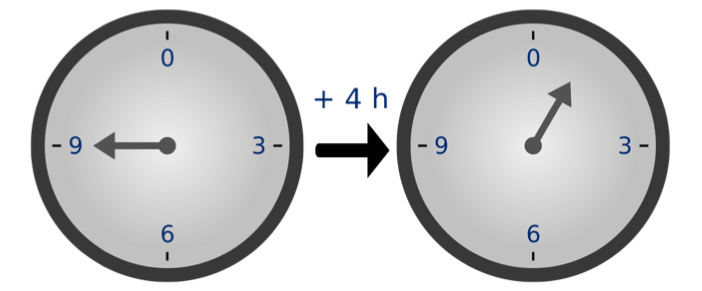
\includegraphics[width=.75\textwidth]{clock.png}
	\caption{Real-life example of modular arithmetic\cite{wiki}.}
	\label{img:clock}
\end{figure}

\begin{teorema}
	Given two integers $a$ and $b$, and a positive one $n$. $a$ and $b$ are said to be \textit{congruent modulo n}, if their difference $a-b$ is an integer multiple of $n$.\\
	The congruence relation is denoted 
	\begin{equation}
	a \equiv b\bmod n
	\end{equation}
\end{teorema}
The integers modulo $m$ are the possible remainders modulo $m$. They are denoted by $\mathbb{Z}_{m}$. The set of integers modulo $m$ is $\mathbb{Z}_{m}$=\{0, 1,$\dots$,m-1\}.

\paragraph{Properties}
Let $a_{1}, a_{2}, b_{1}$ and $b_{2}$ be integers such that $a_{1}\equiv b_{1}\bmod\ n$ and $a_{2}\equiv b_{2}\bmod\ n$. Thus:
\begin{equation}
	a_{1}+a_{2}\equiv b_{1}+b_{2}\bmod\ n
\end{equation}

\begin{equation}
	a_{1}-a_{2}\equiv b_{1}-b_{2}\bmod\ n
\end{equation}

\begin{equation}
	a_{1}a_{2}\equiv b_{1}b_{2}\bmod\ n
\end{equation}
these are, respectively, \textit{addition, subtraction} and \textit{multiplication}.
Moreover,given $a,b$:
\begin{equation}
	(a\bmod\ n)(b\bmod\ n)\equiv (ab)\bmod\ n
\end{equation}

\begin{equation}
	((a\bmod\ n)(b\bmod\ n))\bmod\ n\equiv (ab)\bmod\ n
\end{equation}

\subsection{Groups and Finite Fields}
Cryptography bases its basis also onto groups, rings and finite fields theory.

\begin{teorema}{\textbf{Group (G,*)}}\\
	A set G together with a binary operation $*$, that combines two elements $a$ and $b$ to form another element $a*b$, is a \textit{group} if it satisfies four requirements, known as the \textit{group axioms}:
	\begin{itemize}
		\item \textbf{Closure}: $\forall a,b \in G,\ a*b \in G$.
		\item \textbf{Associativity}: $\forall a,b,c \in G,\ (a*b)*c=a*(b*c)$.
		\item \textbf{Identity}: there exists an unique element $e \in G$ such that, $\forall a\in G$, $a*e=e*a=a$.
		\item \textbf{Invertibility}: $\forall a\in G$ there exists an element $b\in G$ such that, $a*b=b*a=e$.
	\end{itemize}
\end{teorema}

If $\forall a,b\in G$ $a*b=b*a$, $(G,*)$ is a \textit{commutative group}, also known as \textit{Abelian Group}.
\begin{example}
	Integers under addition $(\mathbb{Z},+)$ is an \textit{Abelian Group}; while integers under multiplication $(\mathbb{Z},\times)$ is not even a group.
\end{example}

\begin{example}
	For any modulus $p$ ([0,p-1],+) is a commutative group:
	\begin{itemize}
		\item $0$ is the \textit{identity} element 
		\item $\forall$ a, p-a is the \textit{inverse}
	\end{itemize}
\end{example}

\begin{example}
	For any prime number p ([1,p-1], $\times $) is a commutative group:
	\begin{itemize}
		\item 1 is the identity number
		\item $\forall a$ there exists its inverse, such that $ab\equiv$ 1 mod p	
	\end{itemize}
\end{example}

A group is called finite if it has a finite number of elements. The number of elements is called the \textit{order} of the group.\\

A group is \textit{cyclic} if its elements are \textit{powers} of a particoular one.\\
In this case, the element $g$ is the \textit{generator} of the group.

\begin{teorema}{\textbf{Ring (G,+,$\times$)}}\\
	A set G together with two binary operations (+, $\times$), is a ring if it satisfies the following requirements, the \textit{ring axioms}:
	\begin{itemize}
		\item (G,+) is an abelian group.
		\item (G,$\times$) is a \textit{semigroup}, which basically means that it satisfies the associativity property.
		\item $\times$ is \textit{distributive} with respect to +, it means that $\forall a,b,c \in G$:
		\begin{enumerate}
			\item $a\times (b+c)=(a\times b)+(a\times c)$.
			\item $(a+b)\times c=(a+c)\times (b+c)$.
		\end{enumerate}
	\end{itemize}
\end{teorema}

\begin{teorema}{\textbf{Field $\mathbb{F}$}}\\
	A field $\mathbb{F}$ is a ring such that the second operation satisfies all the group properties for all the elements but the identity element of the first operation.
\end{teorema}

A field which contains a finite number of elements is a \textit{finite field}.




\section{Elliptic Curve}
Now that we have given the preliminary definitions, we can introduce the theory of the Elliptic Curve, which is the basis of this thesis.
\begin{teorema}{(\textbf{Formal definition})}
	In mathematics, an elliptic curve is a plane algebraic curve defined in terms of the Weierstrass equation:
	\begin{equation}
	\label{eqn:EC}
	 y^{2}=x^{3}+ax+b
	\end{equation}
	that is non-singular; that is, it has no cusps or self-intersections.
\end{teorema}

Depending on the value of $a$ and $b$, elliptic curves may assume different shapes on the plane.

\begin{figure}[H]
	\centering
	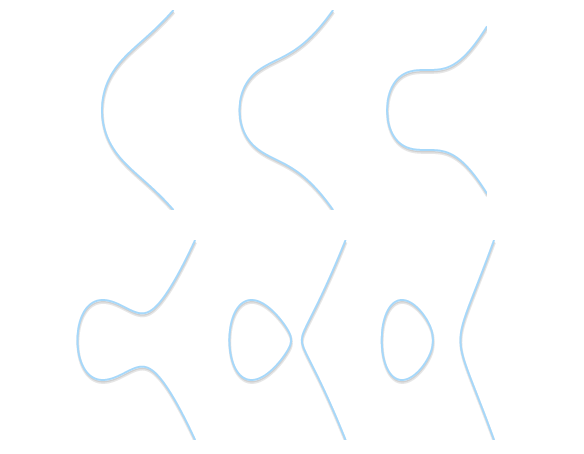
\includegraphics[width=.75\textwidth]{eccurves.png}
	\caption{Examples of elliptic curves\cite{graf}.}
	\label{img:ec_curves}
\end{figure}

The points of an elliptic curve together with the \textit{addition operation, +,} form an \textit{Abelian Group}, where:
\begin{itemize}
	\item \textbf{identity point}: the \textit{point at infinity} $\mathcal{O}$.
	\item \textbf{inverse} of the point $P$: its symmetric about the $x$-axis.
	\item \textbf{addition rule}: give three aligned, non-zero points over the EC $P,Q$ and $R$, $P+Q+R=0$.
\end{itemize}
As this is an abelian group, the addition becomes: $P+Q=-R$. So, in order to compute $P+Q$ you have to draw the line passing through $P$ and $Q$; $R$ is the third intersected point. The result of the addition operation is the inverse of $R$, $-R$.

\begin{figure}[H]
	\centering
	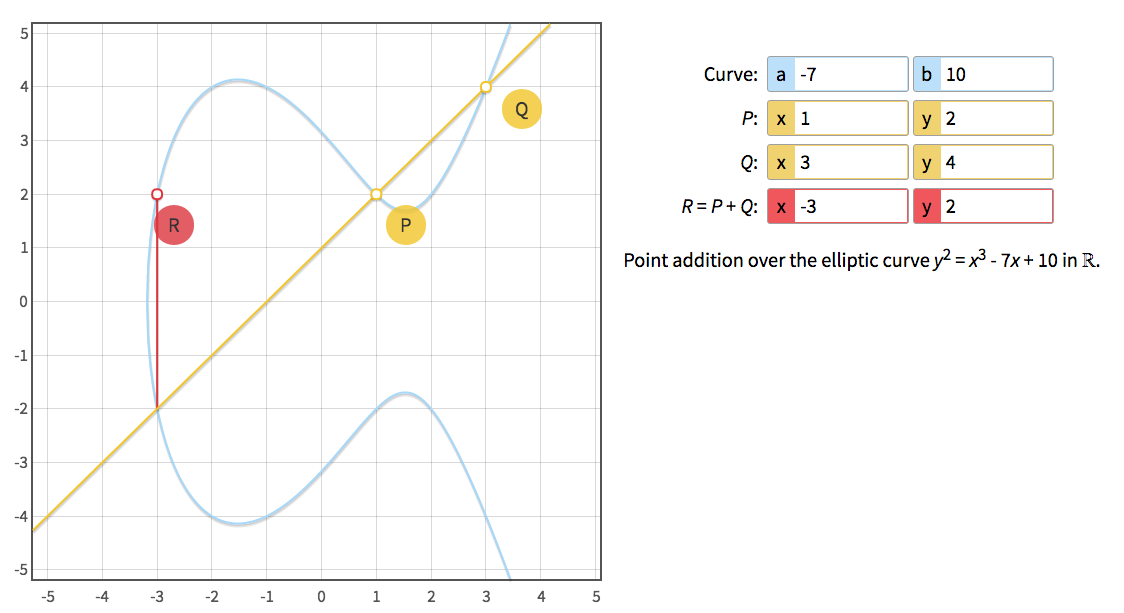
\includegraphics[width=.7\textwidth]{ec_somma.png}
	\caption{Addition\cite{graf}.}
	\label{img:ec sum}
\end{figure}
Formally, we should compute:
\begin{equation}
m=\frac{y_{P}-y_{Q}}{x_{P}-x_{Q}}
\end{equation}

\begin{equation}
x_{R}=m^{2}-x_{P}-x_{Q}
\end{equation}

\begin{equation}
y_{R}=y_{P}+m(x_{R}-x_{P})
\end{equation}

If $P=Q$, you have to draw the tangent to the curve in $Q$.

\begin{figure}[H]
	\centering
	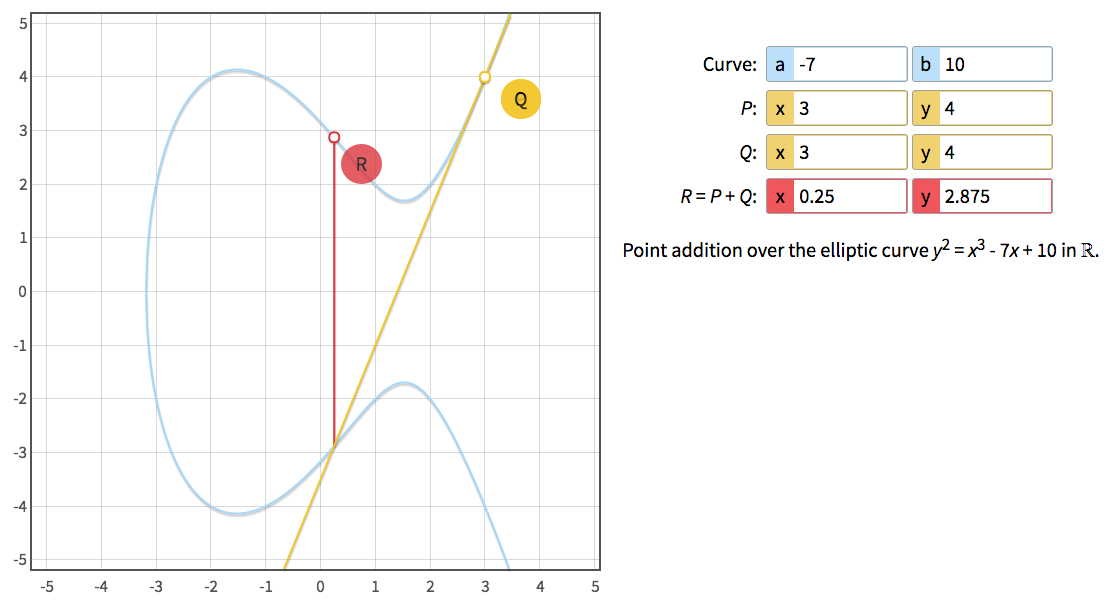
\includegraphics[width=.7\textwidth]{doubling.png}
	\caption{Point Doubling\cite{graf}.}
	\label{img:ec prod}
\end{figure}

If $P\neq Q$ but the line intersects only two points, then the line should be tanget to the curve. $R$ is the inverse of the point of tangency.

\subsection{Over a finite field}
Let \textit{E} be an elliptic curve over a finite field $\mathbb{F}_{p}$, where $p$ is a very high prime number, $p\neq 2,3$. Then, \textit{E} is described by the Equation \eqref{eqn:EC}, where $a,b \in \mathbb{F}_{p}$, such that $4a^{3}+27b^{2}\neq 0$.\\
The last requirement ensures that \textit{E} is non-singular, this means in particular that it is possible to compute the tangent in every point of the curve.\\
The of the \textit{rational points} in \textit{E} over $\mathbb{F}_{p}$, denoted by $E(\mathbb{F}_{p})$, is:
\begin{equation}
	E(\mathbb{F}_{p})=\{(x,y)\in \mathbb{F}_{p}^{2} :\ y^{2}\equiv x^{3}+ax+b (\bmod\ p),\ 4a^{3}+27b^{2}\not\equiv 0\ (\bmod\ p) \}\cup \{\mathcal{O}\}
\end{equation}

\begin{figure}[H]
	\centering
	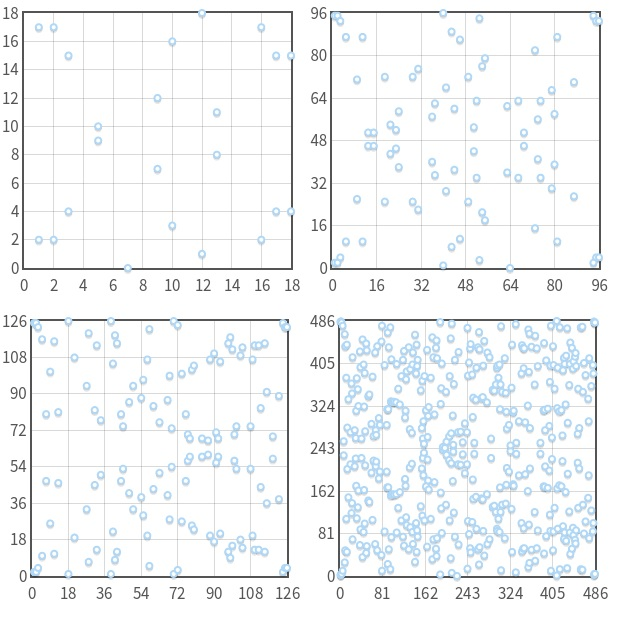
\includegraphics[width=.7\linewidth]{EC_ex.jpg}
	\caption{Examples of Elliptic Curve over Finite Fields\cite{graf}.}
\end{figure}
How does the addition operation changes in a finite field?\\
Informally, we can say that a line in $\mathbb{F}_{p}$ is the set of points $(x,y)$ which satisfy the equation $ax+by+c\equiv 0\ (\bmod\ p)$.
\begin{figure}[H]
	\centering
	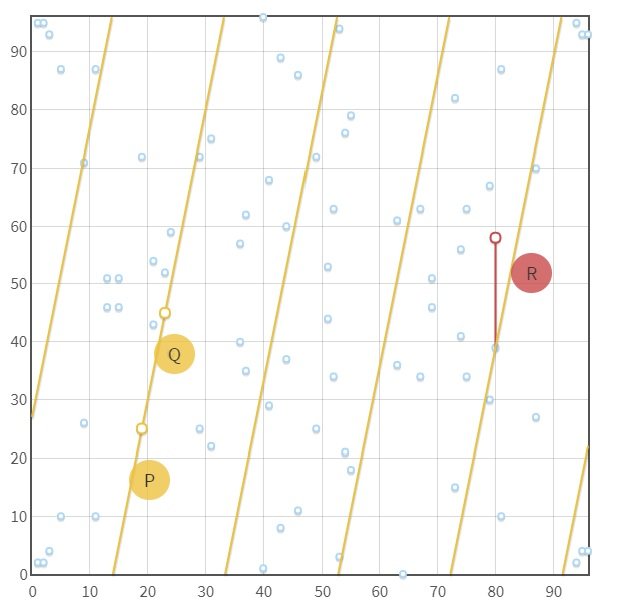
\includegraphics[width=.7\linewidth]{EC_aligned.jpg}
	\caption{Point addition on an EC over a Finite Field\cite{graf}.}
	\label{img:ec-ff}
\end{figure}
Note that the line $y\equiv 4x+83 (\bmod\ 127)$ that connects the points "repeats" itself in the plane.\\
Formally, we should compute:
\begin{equation}
m\equiv \frac{y_{P}-y_{Q}}{x_{P}-x_{Q}} (\bmod\ p),
\end{equation}

\begin{equation}
x_{R}\equiv m^{2}-x_{P}-x_{Q}\ (\bmod\ p),
\end{equation}

\begin{equation}
y_{R}\equiv y_{P}+m(x_{R}-x_{P})\ (\bmod\ p).
\end{equation}

\paragraph{Domain Parameters}
Elliptic curve domain parameters yield a set of information for communicating parties to identify a certain elliptic curve group for use in cryptography. The domain parameters comprise the finite field $\mathbb{F}_{p}$, the coefficients $a$ and $b$ of the $Weierstrass$ equation, a base point $G\in E(\mathbb{F}_{p})$, its order $n$,
and finally the cofactor $h=\frac{\#E(\mathbb{F}_{p})}{n}$. \\
The base point $G$ generates a cyclic subgroup of order $n$ in $E(\mathbb{F}_{p})$ denoted by $\langle{G}\rangle$, i.e.:
$\langle{G}\rangle= \{G, 2G,\dots, (n-1)G\} \cup {\mathcal{O}}$.

\begin{figure}[H]
	\centering
	\begin{tabular}{|l|l|}
		\hline
		\textbf{Parameter} & \textbf{Explanation}\\
		\hline
		\hline
		\textit{p} & A \textit{prime} number specifying the underlying field $\mathbb{F}_{p}$ \\
		\hline
		\textit{a} & The \textit{first} coefficient of Weierstrass equation \\
		\hline
		\textit{b} & The \textit{second} coefficient of Weierstrass equation \\
		\hline
		\textit{G} & The \textit{generator} point \\
		\hline
		\textit{n} & The \textit{order} of $G$ \\
		\hline
		\textit{h} & The \textit{cofactor} of $G$ \\
		\hline
	\end{tabular}
	\caption{Elliptic Curve domain parameters over $\mathbb{F}_{p}$\cite{ECC}.}
	\label{EC:dom par}
\end{figure}


\subsection{Bitcoin's Elliptic Curve}
Bitcoin uses the Koblitz curve \textit{secp256k1}, which has never been used before. It is characterised by the following parameters domain:
\begin{itemize}
	\item $p=FFFFFFFF\ FFFFFFFF\ FFFFFFFF\ FFFFFFFF\ FFFFFFFF\\ FFFFFFFF\ FFFFFFFE\ FFFFFC2F=2^{256}-2^{32}-2^{9}-2^{8}-2^{7}-2^{6}-2^{4}-1$
	\item $a=00000000\ 00000000\ 00000000\ 00000000\ 00000000\ 00000000\ 00000000\ 00000000$
	\item $b=00000000\ 00000000\ 00000000\ 00000000\ 00000000\ 00000000\ 00000000\ 00000007$
	\item $G=04\ 79BE667E\ F9DCBBAC\ 55A06295\ CE870B07\ 029BFCDB\ 2DCE28D9\\ 59F2815B\ 16F81798\ 483ADA77\ 26A3C465\ 5DA4FBFC\ 0E1108A8\ FD17B448\\ A6855419\ 9C47D08F\ FB10D4B8$ (uncompressed)
	\item $n=FFFFFFFF\ FFFFFFFF\ FFFFFFFF\ FFFFFFFE\ BAAEDCE6\\ AF48A03B\ BFD25E8C\ D0364141$
	\item $h=01$
\end{itemize}
So the EC over $\mathbb{F}_{p}$ is:\\ $E(\mathbb{F}_{p})=\{(x,y)\in \mathbb{F}_{p}^{2} :\ y^{2}\equiv x^{3}+7\ (\bmod\ p)\}\cup \{\mathcal{O}\}$.\\
Satoshi Nakamoto chose this curve because is the only one which was generated in a $non-random$ way, so it $30\%$ faster than the others. Moreover, it is defined over a ring, not over a binary Galois field.

\section{Discrete Logarithm}
The Elliptic Curve Cryptography, known as ECC, that is cryptography based on EC, is particularly interesting because it takes advantage of the fact that the Discrete Logarithm Problem (DLP) for EC is proven to be very "hard".
%Indeed it is simple, given $k$ and $P$, to compute $G=kP$
\begin{teorema}
	Let G be a cyclic group of order n with generator g. The discrete logarithm of $h\in G$ to the base g, denoted by $\log_{g} h$, is the unique integer k, $0\leq k \leq n-1$, such that $g^{k}=h$.\\
	Given g and h, the DLP is to find k.
\end{teorema}
The best known algorithms to break the elliptic curve discrete logarithm problem take steps proportional to $\sqrt{2^{n}} = 2^{\frac{n}{2}}$ , where $n$ is the number of bits of the key. \textit{secp256k1} uses 256 bit keys, so the number of steps needed to break it is $2^{128}$.

\section{Hash Function}
\begin{teorema}
	A hash function H is a one-way function that maps data of arbitrary size to a bit string of a fixed size, the hash value or digest.
\end{teorema}
Hash functions have a lot of useful applications in cryptography, such as digital signatures, message authentication, fingerprinting, and so forth.\\
In order to be suitable for cryptography, an hash function has to satisfy the following requirements:
\begin{enumerate}
	\item \textbf{Pre-image resistance}: given an hash value $h$ it is computationally infeasible to find $m$ such that $h=H(m)$.
	\item \textbf{Second pre-image resistance}: given an input $m_{1}$ it is computationally infeasible to find another input $m_{2}\neq m_{1}$, such that $H(m_{1})=H(m_{2})$
	\item \textbf{Collision resistance}: it is computationally infeasible to find two different inputs $m_{1}, m_{2}$, such that $H(m_{1})=H(m_{2})$.
\end{enumerate}

It is important to notice that \textit{Collision resistance} $\Rightarrow$ \textit{Second pre-image resistace}, but $\nRightarrow$ \textit{Pre-image resistance}.
\begin{example}
	One of the most diffused hash function is SHA-1 (produces a 160-bit (20-byte) hash value). It was designed by the United States National Security Agency, and is a U.S. Federal Information Processing Standard. Since 2005 SHA-1 has not been considered secure against well-funded opponents and, in 2017, CWI Amsterdam and Google announced they had performed a collision attack against SHA-1.\\
	So, it is not collision resistant $\Rightarrow$ it is not a good hash function.
\end{example}

Actually, Bitcoin uses SHA-256, which is one of the successor hash functions to SHA-1, and is one of the strongest hash functions currently available.
\paragraph{Properties} 
As we said before, the size of the possible hash values is smaller than the size of possible input data. Therefore, many input data points will share a single hash value output $\Rightarrow$ collisions do exist. But you have to try $2^{130}$ randomly chosen inputs in order to have $99.8 \% $ chance that two of them will collide. So, it is computationally unfeasible.\\
Hence, if we know $h(x) = h(y)$, it is safe to assume that $x= y$.
%\paragraph{Puzzle-friendliness}
%Given $x$ and a target set $Y$, to find $r$ from high min-entropy distribution such that $H(x|r)\in Y$, there is no solving strategy better than trying random values of $r$. (Brute force).\\
%Min-entropy measures how likely you are to guess a value on your first try. If this probability is $p$, then the min-entropy is defined as -$\log_{2} p$.\\
%For example, for a fair coin toss, you'd have $p = 0.5$, giving a min entropy of 1 bit. A uniformly random 256-bit string would have -$\log_{2} 2256 = 256$ bits of min entropy.

An important application of secure hashes is verification of message integrity. Determining whether any changes have been made to a message (or a file), for example, can be accomplished by comparing message digests calculated before, and after, transmission (or any other event).\\
For this reason, most digital signature algorithms only confirm the authenticity of a hashed digest of the message to be "signed". Verifying the authenticity of a hashed digest of the message is considered proof that the message itself is authentic.


\section{Elliptic Curve Cryptography}
In 1985, Neal Koblitz and Victor S. Miller independently proposed to use of the elliptic curves in cryptography. This brought to the birth of Elliptic-curve cryptography (ECC) which is a type of public-key cryptography based on the difficulty of computing discrete logarithms in the group of points on an elliptic curve defined over a finite field. 

\begin{teorema}{(\textbf{Public-key cryptography})}
	Public key cryptography, also known as asymmetric cryptography, is any cryptographic system that uses pairs of keys: \textit{public keys} which can be disclosed, and \textit{private keys} which must be known only by the owner.
\end{teorema}

\subsection{Key pair generation}
\textbf{Inputs:} The elliptic curve domain parameters \textit{(p, a , b, G, n, h)}. \\
\textbf{Actions:} The following actions are performed:

\hspace{1.1cm}
\begin{minipage}[l]{2\linewidth}
	\begin{enumerate}
		\item The \textbf{private key} is: $p=random({1, 2, \dots, n-1})$;
		\item The \textbf{public key} is: $P=p\times G$.\\
	\end{enumerate}
\end{minipage}
\textbf{Output:} $(p,P)$

$P$ is a point on the elliptic curve; while $p$ is an integer, the number of additive steps from the generator point $G$ to arrive at point $P$. \\
Here it becomes clear why it is fundamental that DLP is such a hard problem over elliptic curves! Indeed, the \textit{private key} must be secret, only the owner should know it; while the \textit{public key} can be known by everyone. That is also the reason why the \textit{prime} number of $E$ should be very high:\\
$p$ high $\implies n$ high $\implies$ it is unfeasible to know and try every single number in order to steal the \textit{private} key.
\subsection{Signature Protocol}
Until now, we have been focused on the mathematical structure that allows us to approach this type of cryptogrphy, but how does a signature algorithm work?\\
The scenario is the following: Alice wants to sign a message $m$ with her private key ($p_{A}$), and Bob wants to validate the signature using Alice's public key ($P_{A}$). Nobody but Alice should be able to produce valid signatures. Everyone should be able to check signatures. They are using the same domain parameters.\\
First, Alice generates her key pair and hashes the message, $h=H(m)$. With her private key, she generates her signature over $h$ and sends it to Bob.\\
This last computes $h$ and uses it, together with Alice's public key, in order to verify the validity of the received signature.\\
In the figure below it is represented this process.\\

\begin{figure}[H]
	\centering
	\renewcommand{\arraystretch}{2}
	\begin{tabular}{ccccc}
		\cline{2-2}\cline{4-4}
		 & \multicolumn{1}{|c|}{Message} &  &
		\multicolumn{1}{|c|}{Message}& \\
		\cline{2-2}\cline{4-4}
		 & $\Bigg\downarrow$ & & $\Bigg\downarrow$& \\
		\cline{2-2}\cline{4-4}
		 & \multicolumn{1}{|c|}{Hash Function} &  &
		\multicolumn{1}{|c|}{Hash Function}& \\
		\cline{2-2}\cline{4-4}
		 & $\Bigg\downarrow$ & & $\Bigg\downarrow$& \\
		\cline{2-2}\cline{4-4}
		 & \multicolumn{1}{|c|}{Message Digest} &  &
		\multicolumn{1}{|c|}{Message Digest}& \\
		\cline{2-2}\cline{4-4}
		 & $\Bigg\downarrow$ & & $\Bigg\downarrow$& \\
		\cline{2-2}\cline{4-4}
		$\xrightarrow{Private Key}$ & \multicolumn{1}{|c|}{Signature Generation} & $\xrightarrow[Signature]{Public Key}$&
		\multicolumn{1}{|c|}{Signature Verification}& $\xrightarrow{True/False}$\\
		\cline{2-2}\cline{4-4}
	\end{tabular}
\caption{Signature Process.}
\label{SigProt}
\end{figure}
